\section{Arithmetic objective and source boundary}
The current programme does not yet force a positive integer witness at every
prescribed prime. Its exact receiver and mixed-source fibre theorems begin
with an occupied source. We return to the complete original bounded divisor
boxes, rather than strengthening another post-witness norm estimate.
The basis read for this continuation is the integrated workbench at
\texttt{20709bee872ad10e4cc7d7b976d975e24532a803}. In particular, the redundant
orientation bit removed during integration is not reinstated: an M word
already records its tail order; an E word has its separately retained swap.
The current corrections and the exact scope of the prior inverse are
recorded in the integration audit \citep{Integrated}. The rational trace
relaxation and the earlier residual-divisor maps are inherited from the
pinned mod-24 source \citep[\S\S2--3]{Trace}.

The new results have three components. First, the full square-gate defect is
an additive cyclic coordinate in an explicitly square-zero ideal. Its bounded
multiplicative source has an exact decomposition into finite additive
polynomials, with integer coefficients, stabilizers, and a sharp saturation
criterion. Second, prime-power and prime-square sources admit exact
classifications, including a terminal prime-square middle obstruction to
all existing same-word and same-ray divisor deletions. Third, a different
factor-sum map crosses some of those obstructions and has a complete inverse;
on square carriers its precise arithmetic is a Pell equation. A finite
least-example certificate proves that no universal repair from every trace
can be required to decrease the original distinguished denominator.

No assertion of universal ES, uniform source occupancy, or historical priority
is made. The term ``square-zero'' below refers to the specified finite-ring
ideal. It is not an identification with an independently defined Split-Zero
cohomology class or its support types. The connecting maps to the original
integer coefficients are displayed instead.

\section{Original E/M boxes and rational trace coordinates}\label{sec:source}
Fix a prime $p\equiv1\pmod4$ and an integer $a$ with $p/4<a<p/2$.
Set $R=4a-p$. Then $3\le R<p$, $R\equiv3\pmod4$, and
$\gcd(pa,R)=1$. Every original word is
\[
 a=\prod_{i=1}^n q_i^{e_i},\qquad
 u=\prod_iq_i^{f_i},\qquad0\le f_i\le2e_i.
\]
Write $\beta_i=f_i-e_i$ and normalize
\[
 g=\gcd(a,u),\quad(h,r,s)=(g^2/u,u/g,a/g).
\]
Thus $a=hrs$, $u=hr^2$, $\gcd(r,s)=1$, and the centred prime coordinate is
$\beta_i=v_{q_i}(r)-v_{q_i}(s)$. All following rational triples retain their
order:
\begin{align}
 E:\quad &(a,y,z)=(hrs,hs\kappa,phr\kappa),&
 \kappa&=(pr+s)/R,\label{eq:E}\\
 M:\quad &(a,y,z)=(hrs,phs\lambda,phr\lambda),&
 \lambda&=(r+s)/R.\label{eq:M}
\end{align}
Their reciprocal sum is $4/p$, by multiplying through by $phrs\kappa$ or
$phrs\lambda$. Equivalently the two tails are
\[
 E:\left(\frac{pa+a^2/u}{R},\frac{pa+p^2u}{R}\right),\qquad
 M:\left(\frac{p(a+a^2/u)}{R},\frac{p(a+u)}R\right).
\]
The full gates are $R\mid4u+1$ and $R\mid p+4u$, respectively. The ordered
inverses are $u=a^2/(Ry-pa)$ and $u=pa^2/(Ry-pa)$.
These identities are inherited, not newly discovered here: Yamamoto's
Lemma 2, equation (4), printed p.~38 supplies the exterior congruences
\citep{Yamamoto}; the general Type-I/II representations and their converses
are in \citet[\S2, Propositions 2.2 and 2.6]{ET}.

An explicit crosswalk to their six coordinates is also available. Our full M
state maps to their Type-II sextuple
\[
 (a_{ET},b_{ET},c_{ET},d_{ET},e_{ET},f_{ET})
 =(s,r,\lambda,h,R,4hs\lambda-1).
\]
Their equation (2.22) returns our $(a,y,z)$ without a permutation. Our full E
state maps to their Type-I sextuple
\[
 (r,\kappa,s,h,(r+\kappa)/s,R),
\]
and their projection returns $(z,a,y)$; this cyclic permutation is retained.
For rational traces these parameters need not all be integers.

\begin{lemma}[Complete rational trace source]\label{lem:trace}
Put $G_E=4u+1$, $G_M=p+4u$. The corresponding two tails have integral sum
exactly when $R\mid G_c^2$. Their common reduced denominator is
$d=R/\gcd(R,G_c)$; on a trace, $d^2\mid R$.
Every positive rational pair $(y,z)$ at this integral $a$ satisfying
\[
 \frac4p=\frac1a+\frac1y+\frac1z
\]
and having integral sum $y+z$ occurs in these coordinates, with the E swap
retained.
\end{lemma}
\begin{proof}
The sums are $(a+pu)^2/(Ru)$ and $p(a+u)^2/(Ru)$. Since $u\mid a^2$ and
all $p,a,u$ are units modulo $R$, their integrality gives the square gates.
The gcds of the two integral numerators with $R$ agree and give the stated
common denominator.
Conversely, if $N=y+z\in\mathbb Z$, the reduced denominators of $y,z$ coincide
at $d$. Their product $yz=Npa/R$ has reduced denominator $d^2$, since the
reduced numerators of both tails are units at every prime dividing $d$.
Hence $d^2=R/\gcd(R,N)$, and $d\mid R$.
The numbers $b=Ry-pa$, $c=Rz-pa$ are positive integers satisfying
$bc=(pa)^2$. Their $p$-valuation pair is $(0,2),(1,1)$, or $(2,0)$.
For $(0,2)$ take $u=a^2/b$; for $(2,0)$ first exchange the tails; for
$(1,1)$ take $u=pa^2/b$. These are precisely the original words and formulas.
\end{proof}

\begin{lemma}[Character parity]\label{lem:char}
For an original trace,
\[
 E:\ (u/p)=-1,\qquad M:\ (u/p)=-(a/p).
\]
Here the symbols are Legendre symbols at $p$; Jacobi symbols at $R$ are used
only inside the proof.
\end{lemma}
\begin{proof}
For odd $q_i\mid a$, reciprocity and $R\equiv-p\pmod{q_i}$ give
$(q_i/R)=(p/q_i)=(q_i/p)$. At two the supplementary law and
$R\equiv-p\pmod8$ give the same equality. Multiplication through all original
exponents proves $(u/R)=(u/p)$ and $(a/R)=(a/p)$.
The square gate implies the unsquared gate at every prime dividing $R$, not
necessarily modulo $R$. It suffices for its Jacobi value, with all prime
multiplicities retained. Since $(-1/R)=-1$ and
$(p/R)=(R/p)=(a/p)$, the E normalized residue $pu/a$ has Jacobi value
$(u/p)$; the M residue $u/a$ has value $(u/p)(a/p)$. Both must equal $-1$.
\end{proof}

\section{A square-zero additive defect on the entire source}\label{sec:defect}
Define
\[
 K=\prod_{\ell^v\parallel R}\ell^{\lceil v/2\rceil},\quad
 D=R/K,\quad \delta=R/D^2.
\]
Then $R=KD=\delta D^2$, $D\mid K$, and $\delta$ is the positive squarefree
part, not the radical. Also $\delta\equiv3\pmod4$, hence
\begin{equation}\label{eq:D-bound}
 D\le\sqrt{R/3}<\sqrt{p/3}.
\end{equation}
The ideal $J=K\mathbb Z/R\mathbb Z$ obeys $J^2=0$, because $R\mid K^2$.
The map $\mathbb Z/D\to J$, $c\mapsto Kc$, is an additive isomorphism.

For channel exponent $\eta=1$ in E and $\eta=0$ in M, put
\[
 z_{\eta,\beta}=p^\eta\prod_iq_i^{\beta_i}=p^\eta u/a
 \quad\text{in }(\mathbb Z/R\mathbb Z)^\times.
\]
Trace is exactly $z\equiv-1\pmod K$. Thus it has a unique coordinate
\begin{equation}\label{eq:defect}
 z=-1+Kc,\qquad c\in\mathbb Z/D.
\end{equation}
The full gate is $c=0$, and the actual common tail denominator is
\begin{equation}\label{eq:denorder}
 d=\frac{D}{\gcd(D,c)}.
\end{equation}
Indeed the two normalized residues are unit multiples of their original gates,
so $\gcd(R,G_c)=\gcd(R,z+1)=K\gcd(D,c)$.
The case $D=1$ is retained: its defect group is trivial and every trace is full.

\begin{theorem}[Mixed integer-exponent law]\label{thm:mixed}
Take original traces $(\eta_j,\beta^{(j)},c_j)$ at a common $(p,a,R)$.
Let $n_j\in\mathbb Z$, with
\[
 N=\sum_jn_j\text{ odd},\qquad
 \eta_* =\sum_jn_j\eta_j\in\{0,1\},\qquad
 \beta_* =\sum_jn_j\beta^{(j)}\in\prod_i[-e_i,e_i].
\]
Then this is an original trace in channel $\eta_*$, with
\begin{equation}\label{eq:mixed}
 u_*=a^{1-N}\prod_j u_j^{n_j},\qquad
 c_*=\sum_jn_jc_j\pmod D.
\end{equation}
It is a full original state exactly when the latter sum is zero.
\end{theorem}
\begin{proof}
Write $z_j=-(1-Kc_j)$. In the square-zero ideal,
$(1-Kc_j)^{n_j}=1-n_jKc_j$ for every integer exponent, including negative
ones. Their product, since $N$ is odd, is
$-1+K\sum n_jc_j$. Its channel and prime exponents are precisely the displayed
ones. The bounded exponent requirement proves that $u_*$ is a positive integer
divisor of $a^2$, rather than an arbitrary unit residue. Apply
\eqref{eq:E}--\eqref{eq:M} and their ordered inverses.
\end{proof}

In particular E$_1-$E$_2+$M returns M when its original box permits it:
\[
 u_*=u_{E,1}u_M/u_{E,2},\qquad c_*=c_{E,1}-c_{E,2}+c_M.
\]
Retaining the two other inputs gives an inverse for this ternary map.
For a general coefficient vector, the complete fibres are the bounded integer
solutions of the displayed linear equations in the $\beta^{(j)}$ and their
channel exponents, within their stated original trace domains; no assertion of injectivity after forgetting inputs is made.

\subsection{Every coarse-neutral line has an exact finite return}
Let $\gamma\in\mathbb Z^n$ satisfy
$\phi(\gamma)=\prod q_i^{\gamma_i}\equiv1\pmod K$. Put
\[
 \lambda_\gamma=(\phi(\gamma)-1)/K\pmod D.
\]
The quotient is well-defined by first evaluating $\phi$ modulo $R$.
For $\beta(t)=\beta_0+t\gamma$ in the original box,
\begin{equation}\label{eq:line}
 c(t)=c_0-\lambda_\gamma t\pmod D.
\end{equation}
The integer interval $L\le t\le U$ is the intersection of the inequalities
$-e_i\le\beta_{0i}+t\gamma_i\le e_i$, using exact floors and ceilings.
For $g=\gcd(\lambda_\gamma,D)$ there is no full state if $g\nmid c_0$.
Otherwise, put $m=D/g$ and
$t_0=(c_0/g)(\lambda_\gamma/g)^{-1}\pmod m$ (take $t_0=0$ for $m=1$).
All full states are exactly $t=t_0+jm$ in $[L,U]$, and their number is
\[
 \max\left(0,\left\lfloor\frac{U-t_0}{m}\right\rfloor
             -\left\lceil\frac{L-t_0}{m}\right\rceil+1\right).
\]
This proves termination on the given line. It does not assert that an arbitrary
line contains a full period or even a trace.

\subsection{A mixed return where every individual deletion fails}
At $p=48049$, take $a=12019=7\cdot17\cdot101$, $R=27$, $K=9$, $D=3$.
The three proper traces are
\[
\begin{array}{c|r|c|c|c}
\text{channel}&u&\beta_{7,17,101}&(h,r,s)&c\\\hline
E&29189&(-1,1,0)&(101,17,7)&1\\
E&119&(0,0,-1)&(119,1,101)&2\\
M&707&(0,-1,0)&(707,1,17)&1.
\end{array}
\]
All tails have common denominator three. E$_1-$E$_2+$M lies in the original
box and gives $u_*=173417$, $\beta_*=(-1,0,1)$ and $c_*=0$. Its marking is
$(h,r,s,\lambda)=(17,101,7,4)$, with
\begin{equation}\label{eq:48049}
 \frac4{48049}=\frac1{12019}+\frac1{22871324}+\frac1{330000532}.
\end{equation}
For each individual trace, both the inherited fixed-word modulus $4K(u)$
and the ray modulus $4rs$ exceed $R$; hence no proper residual-divisor deletion
can be one modulo either modulus. The mixed operation changes the available
word inside the old box instead.
Its neutral-line version has $\gamma=(-1,1,1)$, $\lambda_\gamma=1\pmod3$,
$t\in\{0,1\}$, and $c(t)=1-t$. The actual short interval already contains
its full state; no abstract subgroup replacement is needed.

\begin{figure}[htbp]
\centering
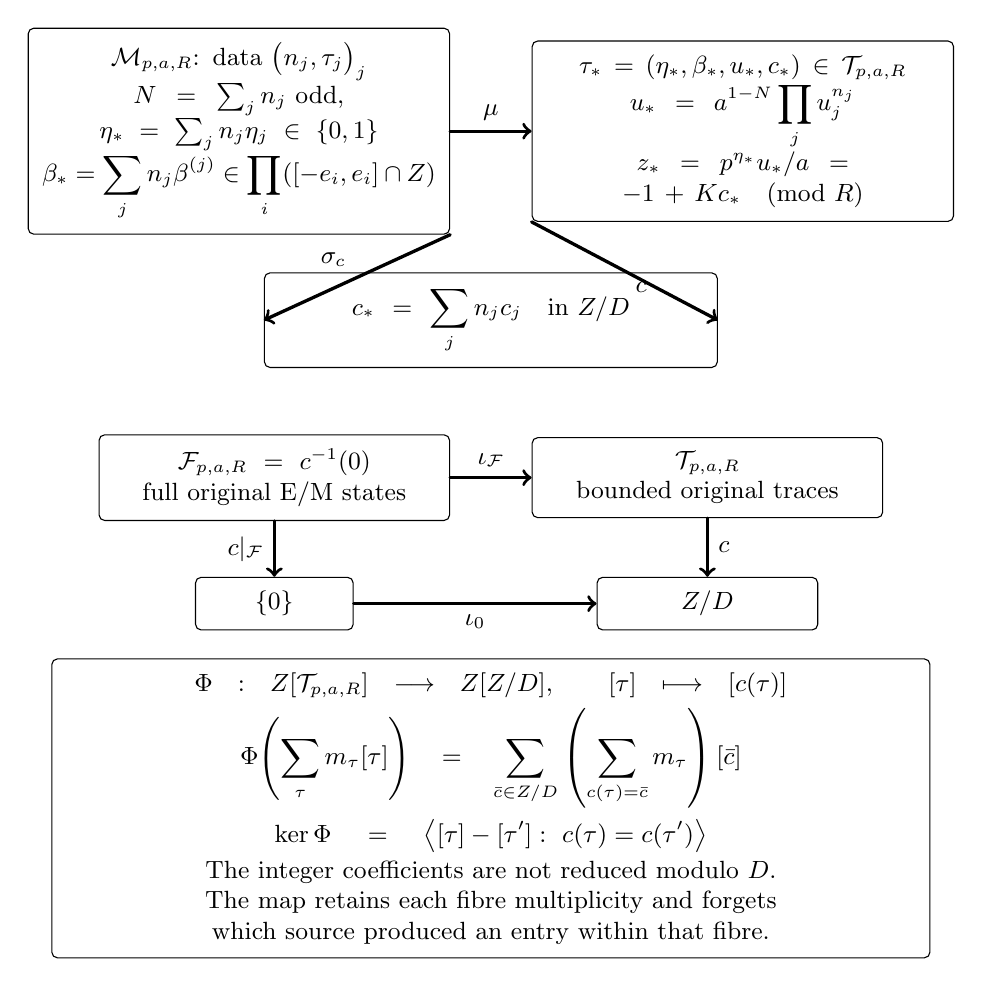
\begin{tikzpicture}[
  font=\small,
  box/.style={draw,rounded corners=2pt,align=center,inner sep=5pt},
  every path/.style={line cap=round,line join=round}
]
  \node[box,text width=5.0cm] (mix) at (-3.2,4.35)
    {$\mathcal M_{p,a,R}$: data $\bigl(n_j,\tau_j\bigr)_j$\\
     $N=\sum_j n_j$ odd,\quad
     $\eta_*=\sum_jn_j\eta_j\in\{0,1\}$\\
     $\displaystyle
       \beta_*=\sum_jn_j\beta^{(j)}
       \in\prod_i([-e_i,e_i]\cap\mathbb Z)$};
  \node[box,text width=5.0cm] (trace-star) at (3.2,4.35)
    {$\tau_*=(\eta_*,\beta_*,u_*,c_*)
       \in\mathcal T_{p,a,R}$\\
     $\displaystyle u_*=a^{1-N}\prod_j u_j^{n_j}$\\
     $z_*=p^{\eta_*}u_*/a=-1+Kc_*\pmod R$};
  \node[box,text width=5.4cm] (defect-sum) at (0,1.95)
    {$\displaystyle c_*=\sum_jn_jc_j\quad\hbox{in }\mathbb Z/D$};

  \draw[->,very thick] (mix) -- node[above]
    {$\mu$} (trace-star);
  \draw[->,very thick] (mix.south east) -- node[above left]
    {$\sigma_c$} (defect-sum.west);
  \draw[->,very thick] (trace-star.south west) -- node[below right]
    {$c$} (defect-sum.east);

  \node[box,text width=4.1cm] (full) at (-2.75,-0.05)
    {$\mathcal F_{p,a,R}=c^{-1}(0)$\\
     full original E/M states};
  \node[box,text width=4.1cm] (traces-fibre) at (2.75,-0.05)
    {$\mathcal T_{p,a,R}$\\bounded original traces};
  \node[box,text width=1.65cm] (zero) at (-2.75,-1.65)
    {$\{0\}$};
  \node[box,text width=2.45cm] (defect-fibre) at (2.75,-1.65)
    {$\mathbb Z/D$};
  \draw[->,very thick] (full) -- node[above]
    {$\iota_{\mathcal F}$} (traces-fibre);
  \draw[->,very thick] (full) -- node[left]
    {$c|_{\mathcal F}$} (zero);
  \draw[->,very thick] (traces-fibre) -- node[right]
    {$c$} (defect-fibre);
  \draw[->,very thick] (zero) -- node[below]
    {$\iota_0$} (defect-fibre);

  \node[box,text width=10.8cm] (module) at (0,-4.25)
    {$\displaystyle
      \Phi:\mathbb Z[\mathcal T_{p,a,R}]
      \longrightarrow\mathbb Z[\mathbb Z/D],\qquad
      [\tau]\longmapsto[c(\tau)]$\\[3pt]
     $\displaystyle
      \Phi\!\left(\sum_{\tau}m_\tau[\tau]\right)
      =\sum_{\bar c\in\mathbb Z/D}
       \left(\sum_{c(\tau)=\bar c}m_\tau\right)[\bar c]$\\[3pt]
     $\displaystyle
      \ker\Phi=
      \left\langle[\tau]-[\tau']:\ c(\tau)=c(\tau')\right\rangle$\\[2pt]
     The integer coefficients are not reduced modulo $D$.
     The map retains each fibre multiplicity and forgets which source produced
     an entry within that fibre.};
\end{tikzpicture}
\caption{Typed maps for the defect equation
$p^\eta u/a=-1+Kc\pmod R$.  In the upper triangle,
$\sigma_c((n_j,\tau_j)_j)=\sum_jn_jc_j$, and the triangle commutes by the
mixed integer-exponent law.  The middle square identifies the
full states as the zero fibre.  The lower map states the exact kernel and the
information lost when original trace words are replaced by their defect-bin
coefficient vector.}
\label{fig:defect-map}
\end{figure}


\section{Complete bounded additive polynomials and sharp saturation}\label{sec:tiles}
For each original prime $q_i\mid a$, set $o_i=\operatorname{ord}_K(q_i)$.
Partition its actual interval $[-e_i,e_i]\cap\mathbb Z$ by residue modulo $o_i$.
Every nonempty part has the unique form
\[
 \beta_i=b_i+o_i t_i,\qquad0\le t_i<N_i,
\]
where $b_i$ is its smallest member. Taking products of these parts partitions
\emph{every} original exponent vector once. Retain separately the channel.

A product part is a coarse trace part exactly when
$p^\eta\prod q_i^{b_i}\equiv-1\pmod K$. Let $c_0$ be its defect and put
\[
 \lambda_i=(q_i^{o_i}-1)/K\pmod D.
\]
Every point of that part has defect
$c_0-\sum_i\lambda_it_i$. Consequently its number of full original words is
\begin{equation}\label{eq:tilepoly}
 \operatorname{coeff}_{c_0}(\mathcal C),
 \qquad
 \mathcal C=\prod_i\left([0]+[\lambda_i]+\cdots+[(N_i-1)\lambda_i]\right)
 \in\mathbb Z[\mathbb Z/D].
\end{equation}
Here $\operatorname{coeff}_{c_0}$ extracts the coefficient of the basis
element $[c_0]$. These are geometric factors with the original coefficient one per exponent,
not binomial factors from artificially distinguished prime occurrences.
The inverse reads $\beta_i$, its part $b_i$, and
$t_i=(\beta_i-b_i)/o_i$; the original word is $\prod q_i^{e_i+\beta_i}$.
Thus \eqref{eq:tilepoly} is an exact arithmetic refinement of the full box.

The homomorphism on free abelian modules sends each original basis word to
its defect-bin basis. Over its actual occupied bins, its kernel has the usual
basis of differences of original words in the same fibre. An empty zero bin
is different from a nonzero integer coefficient reducing to zero modulo a
prime. No coefficient is reduced modulo $D$; only its \emph{index} is.

\begin{theorem}[Unit-direction saturation]\label{thm:saturation}
Suppose $D>1$ and let $U_0=\{i:\gcd(\lambda_i,D)=1\}$. If
\begin{equation}\label{eq:width}
 \sum_{i\in U_0}(N_i-1)\ge D-1,
\end{equation}
then every coefficient of $\mathcal C$ is at least
$\prod_{i\notin U_0}N_i$. In particular the original box part contains at
least that many full states. The number $D-1$ cannot be lowered, even for
packets inside actual hard-prime sources.
\end{theorem}
\begin{proof}
For a nonempty proper subset $S\subset\mathbb Z/D$ and a unit $\lambda$,
$S+\lambda=S$ would make $S$ invariant under a generator and hence the whole
group. Therefore $|S\cup(S+\lambda)|\ge|S|+1$.
Adding successively $N_i-1$ copies of each unit step expands the possible
sumset until it is all of $\mathbb Z/D$ after at most $D-1$ steps.
This repeated-binary description is used only to prove equality of supports:
the possible totals in coordinate $i$ are still $0,\ldots,N_i-1$, each
counted by the original geometric factor. Thus each residue has at least one
original unit-coordinate vector. For each of the
$\prod_{i\notin U_0}N_i$ choices of other coordinates, translate the required
unit residue. The resulting full original vectors are distinct.
A single interval of length $D-1$ and unit step misses one residue, proving
abstract sharpness. The next paragraph realizes that obstruction arithmetically.
\end{proof}

Fix a prime $\ell\equiv3\pmod4$, put $R=\ell^3$, and choose a prime $q>7$
with $q\equiv-1+\ell^2\pmod{\ell^3}$. This reduced progression contains
infinitely many primes by Dirichlet's theorem \citep[Theorem 18.1]{Dirichlet}.
Set $e=\ell-1$. Choose primes $p>R$ satisfying
\[
 p\equiv1\pmod{840},\qquad
 p\equiv-R+4q^e\pmod{q^{e+1}}.
\]
These are compatible reduced conditions, since $q>7$ and $q\nmid R$; another
application of Dirichlet gives infinitely many such primes. An optional
condition $p\equiv1\pmod\ell$ when $\ell\nmid840$ remains reduced as well.
Then $a=(p+R)/4=q^eh$ with $q\nmid h$. Hold every other centred exponent at
zero and vary $\beta_q\in[-e,e]$. Modulo $K=\ell^2$, the M traces are exactly
the odd $\beta_q$. Modulo $R$, their residues are
\[
 q^{\beta_q}=-1+\ell^2\beta_q,
\]
including negative exponents. Their defects run exactly through all nonzero
classes modulo $D=\ell$. This original one-coordinate packet has $N=\ell-1$, unit step
$\lambda=-2$, and width $D-2$, with no full word. Other words at the
same shell may be occupied; none is deleted by this sharpness assertion.

\subsection{Actual coefficient stabilizers}
Write $\mathcal C=\sum_j C_j[j]$. At frequency $k\in\mathbb Z/D$, its Fourier
coefficient is nonzero exactly when, for every $i$,
\[
 D\mid k\lambda_i
 \quad\text{or}\quad D\nmid k\lambda_iN_i.
\]
Indeed a finite geometric sum is zero precisely when its ratio is nontrivial
but its $N_i$th power is one. Let $\mathcal F$ be the displayed nonzero
frequency set, and $g=\gcd(D,\{k:k\in\mathcal F\})$. Fourier inversion gives
\begin{equation}\label{eq:stabilizer}
 \operatorname{Stab}(C)=\{0,D/g,2D/g,\ldots,(g-1)D/g\}.
\end{equation}
This is the stabilizer of the actual coefficient vector, not merely its
support. It includes every multiplicity and is verified against direct shifts
in the executable tables.

\section{Prime powers and the complete prime-square obstruction}\label{sec:squares}
\begin{proposition}[Prime-power M classification]\label{prop:power}
Let $p\equiv1\pmod{24}$, $a=q^e$, $q>3$ prime, and suppose an M trace exists.
Then $(q/p)=-1$. Write $\operatorname{ord}_K(q)=2b$. One has $b$ odd and
$q^b=-1\pmod K$. Put
\[
 d_b=R/\gcd(R,q^b+1),\qquad B=bd_b.
\]
The complete centred trace exponents are the odd multiples of $b$ in $[-e,e]$;
the full exponents are the odd multiples of $B$. Their counts are
\[
 2\left\lfloor\frac{e+b}{2b}\right\rfloor,
 \qquad2\left\lfloor\frac{e+B}{2B}\right\rfloor.
\]
At exponent $bm$ with $m$ odd, the common tail denominator is
$d_b/\gcd(d_b,m)$.
\end{proposition}
\begin{proof}
Lemma~\ref{lem:char} gives $(q/p)^{f-e}=-1$, so $q$ is a nonresidue and
$\beta=f-e$ is odd. In the cyclic subgroup generated by $q\bmod K$, the
presence of $-1$ makes it the unique order-two element, reached at half the
order. Hence every trace exponent is an odd multiple of $b$, and $b$ is odd.
The square-zero law gives $q^b=-1+Kc$, with additive order of $c$ equal to
$d_b$. Thus $q^{2b}=1-2Kc$ has order $d_b$, since $D$ is odd, and
$\operatorname{ord}_R(q)=2bd_b$. Also $q^{bd_b}=-1$ because $d_b$ is odd.
This proves the full exponent description and the denominator formula.
Counting positive and negative odd multiples gives the two displayed counts.
\end{proof}

\begin{theorem}[Complete prime-square trace classification]\label{thm:square}
Let $p\equiv1\pmod{24}$, $q>3$ prime and $a=q^2$ in the first-half range.
A trace forces $q\equiv2\pmod3$. There are exactly four possible marked states:
\[
\begin{array}{c|c|c|c}
\text{channel}&u&\text{trace condition}&\text{full condition}\\\hline
E&q&K\mid4q+1&R\mid4q+1\\
E&q^3&K\mid4q^3+1&R\mid4q^3+1\\
M&q&K\mid q+1&R\mid q+1\\
M&q^3&K\mid q+1&R\mid q+1.
\end{array}
\]
E and M traces coexist only at $R=3$, where all four are full. Both E traces
coexist only at $R=3$ or $75$. At $R=75$ this occurs exactly when
$q\equiv11\pmod{15}$; the low E state is full only at $q\equiv56\pmod{75}$,
and the high one only at $q\equiv11\pmod{75}$.
Every proper M trace has both full original gates empty at its entire shell.
\end{theorem}
\begin{proof}
Since $q^2\equiv1\pmod{24}$, $R\equiv3\pmod{24}$ and $3\mid K$.
If $q\equiv1\pmod3$ no word passes either coarse gate. Otherwise each gate
forces an odd exponent $f$, leaving exactly $f=1,3$ in the full box
$0\le f\le4$. For M these both reduce, by cancellation of a power of $q$,
to $q+1$, proving the table.
If M and either E coexist, reduction at $q=-1\pmod K$ forces $K\mid3$;
$R\equiv3\pmod{24}$ then gives $R=3$. If both E states coexist, the identity
\[
 16(4q^3+1)-(4q+1)(16q^2-4q+1)=15
\]
forces $K\mid15$. Enumerating the possible exponents of three and five
(each at most two in $R$) with $R\equiv3\pmod{24}$ gives $R=3,75$.
At 75 the five classes $q\equiv11,26,41,56,71\pmod{75}$ give the stated
full-gate alternatives by substitution. A proper M trace cannot have $R=3$,
so no E trace coexists; its two M orientations are both nonintegral.
\end{proof}

\begin{theorem}[Terminality for the inherited deletion systems]\label{thm:terminal}
For a proper M trace of Theorem~\ref{thm:square}, neither original word has a
same-word residual-divisor return. Neither corresponding primitive M ray has
a ray-preserving residual-divisor return. These claims retain every divisor of
$R$, not only its prime factors or squarefree part.
For a proper low E trace $u=q$, the complete nontrivial same-word deletion set
is $\{4q+1\}$ if $4q+1\mid R$, and is empty otherwise.
\end{theorem}
\begin{proof}
For $u=q^3$, the same-word modulus is $4q^2>R$, so no proper divisor of $R$
is one modulo that modulus. For $u=q$, both word and M-ray budgets are $4q$.
Any permitted $k>1$ divides $R\mid(q+1)^2$ and is one modulo $4q$.
Its complement $v=(q+1)^2/k$ is an integer one modulo $q$ and exceeds one:
$v=1$ would make $k$ even. Write $k=1+qA$, $v=1+qB$ with $A\ge4,B\ge1$.
Then $qAB+A+B=q+2$, an impossibility. The same $4q$ budget controls the
opposite primitive ray, so it is also excluded.
For low E replace $q+1$ by $m+1$, $m=4q$. If $k>1$ divides
$R\mid(m+1)^2$ and $k\equiv1\pmod m$, then its complement is also one
modulo $m$ and exceeds one, because $R<2q^2<(m+1)^2$.
Writing the two factors as $1+mA,1+mB$ forces
$mAB+A+B=m+2$, whence $A=B=1$. Thus $k=4q+1$ is the sole possibility.
If it divides $R$, write $R=(4q+1)v$. Then $v\mid4q+1$ and the deletion
has full target gate at $v$. Its distinguished denominator is $q(q-v)$ and
its retained word is $q$, proving sufficiency.
\end{proof}

\section{A different arithmetic arrow: retain the factor sum}\label{sec:shift}
The terminality theorem does not prohibit changing both the numerical word
and the primitive ray. The following arrow does exactly that.
Its completeness is relative to the displayed residual $\delta$, unchanged
raw factor $r$, and opposite shifts of $h$ and $s$; it is not a classification
of every possible source-changing map.

\begin{theorem}[Complete factor-sum return and inverse]\label{thm:sumshift}
Take any oriented original M trace
\[
 a=hrs,\quad u=hr^2,\quad \gcd(r,s)=1,\quad
 R=4hrs-p=\delta t^2,\quad \delta t\mid r+s.
\]
Its targets with residual $\delta$, unchanged raw factor $r$, and
\[
 h'=h-\delta w,\qquad s'=s+\delta w,\qquad w\in\mathbb Z
\]
are precisely the integer roots of
\begin{equation}\label{eq:quad}
 r\bigl(\delta w^2+(s-h)w\bigr)=\frac{t^2-1}{4}.
\end{equation}
For such a root set $c=\gcd(r,s')$. Every root gives positive integers $h',s'$
and the full primitive middle marking
\begin{equation}\label{eq:shiftout}
 \begin{gathered}
 a'=h'rs'=(p+\delta)/4,\qquad u'=h'r^2,\\
 (h_M,r_M,s_M,\lambda_M)
 =\left(h'c^2,r/c,s'/c,(r+s')/(c\delta)\right).
 \end{gathered}
\end{equation}
Writing $\lambda'=(r+s')/\delta=c\lambda_M$, its ordered denominators are
\begin{equation}\label{eq:shiftden}
 (h'rs',\ ph's'\lambda',\ ph'r\lambda').
\end{equation}
For a proper trace, $a'<a$.
There are no roots unless $r\mid(t^2-1)/4$. When that holds, there are at most
two, tested by the square discriminant $(h-s)^2+(R-\delta)/r$ and integer
divisibility of $h-s\pm\sqrt{(h-s)^2+(R-\delta)/r}$ by $2\delta$.

For any marked full primitive target $(p,\delta,h_0,r_0,s_0,\lambda_0)$ with
squarefree residual $\delta$, its complete incoming fibre is as follows.
Choose each $c>0$ with $c^2\mid h_0$ and put
\[
 h'=h_0/c^2,\qquad r=cr_0,\qquad s'=cs_0.
\]
For each integer
\begin{equation}\label{eq:inverse-w}
 -h'/\delta<w<s'/\delta,
\end{equation}
retain it precisely when
\[
 t^2=1+4r w(s'-h')-4r\delta w^2
\]
is a positive odd square, $\delta t^2<p$, and
\[
 \gcd(r,s'-\delta w)=1,\qquad
 \delta t\mid r+s'-\delta w.
\]
Recover $h=h'+\delta w$, $s=s'-\delta w$, $a=hrs$, $R=\delta t^2$, $u=hr^2$.
Retaining $(c,w)$ makes the two constructions inverse.
\end{theorem}
\begin{proof}
Multiplication gives
$h'rs'=hrs+r\delta w(h-s)-r\delta^2w^2$.
Requiring $4h'rs'-p=\delta$ is precisely \eqref{eq:quad}.
Its target product $h's'=(p+\delta)/(4r)$ is positive and the factor sum
remains $h+s>0$; hence both factors are positive.
Since $\delta\mid r+s$ and $s'=s+\delta w$, the full raw M gate holds.
The old $r$ is a unit modulo $\delta$, so $c=\gcd(r,s')$ is also a unit there.
Since $c\mid r+s'$, the quotient $(r+s')/(c\delta)$ is an integer.
The displayed primitive normalization follows directly from $c$ and gives
exactly the same ordered denominators. The word $u'=h'r^2$ divides $a'^2$,
with complementary divisor $h's'^2$. Its original first-half range follows
from $3\le\delta<p$. Properness implies $t>1$ and
$a-a'=\delta(t^2-1)/4>0$.
The divisibility by $r$ and discriminant test are exactly the quadratic
formula, retaining every denominator.

Conversely, a primitive target has $h_0=h'c^2$, $r_0=r/c$, $s_0=s'/c$;
thus every lost gcd is among the finite list $c^2\mid h_0$.
For each, positivity of the source factors is \eqref{eq:inverse-w}.
Multiplication gives exactly the displayed $t^2$.
The remaining finite tests are precisely source coprimality, the original
trace gate, and the first-half range. They are therefore sufficient and
necessary. Because $\gcd(r_0,s_0)=1$, the raw target gcd is exactly $c$,
so both compositions recover $(c,w)$ and every original coordinate.
\end{proof}

The source is oriented. Complementing the input word need not preserve this
particular arrow; it changes which raw factor is fixed. An initial
complement followed by the theorem and a target complement is a separately
marked composite. It is not counted as an extra unconstrained orientation
bit on an already ordered source. The theorem changes the numerical word
and generally the primitive ray, so it is neither inherited deletion system.

At the hard prime $p=2003761\equiv361\pmod{840}$, take
\[
 a=501034=2\cdot479\cdot523,\quad R=375=15\cdot5^2,
 \quad u=1916,\quad(h,r,s)=(479,2,523).
\]
Both full original gates at this shell are empty. The source has common
denominator five. Equation \eqref{eq:quad} has $w=-3$, yielding raw target
$(h',r,s')=(524,2,478)$ and gcd $c=2$. Its primitive marking is
\[
 (h_M,r_M,s_M,\lambda_M)=(2096,1,239,16),
\]
with
\[
 \frac4{2003761}
 =\frac1{500944}+\frac1{16060352806144}+\frac1{67198128896}.
\]
The whole incoming fibre of this marked target has three $(w,c)$ pairs:
$(0,1)$, $(-3,2)$ and $(55,4)$. Forgetting the gcd would lose the selected
source and would incorrectly describe the other two preimages.

\subsection{The prime-square specialization is exactly Pell}
If $r=1$ and $h=s=q$, equation \eqref{eq:quad} becomes
\begin{equation}\label{eq:Pell}
 t^2-4\delta w^2=1.
\end{equation}
This gives a completely explicit integer family, not only a test at an
unidentified source. Take $\delta\ge3$ squarefree, $\delta\equiv3\pmod4$,
positive integers $t,w$ satisfying \eqref{eq:Pell}, and $k\ge1$. Put
\begin{equation}\label{eq:Pellsource}
 q=\delta tk-1,\quad p=4q^2-\delta t^2,
 \quad a=q^2,
\end{equation}
then
\begin{equation}\label{eq:Pellout}
 h'=q-\delta w,\qquad s'=q+\delta w,\qquad
 \lambda'=tk+w.
\end{equation}
One has $\gcd(q,\delta t)=1$, $p>\delta t^2>0$, $p\equiv1\pmod4$, and the
full ordered identity \eqref{eq:shiftden}. To check the strict inequality,
$q\ge\delta t-1$ and
$2(\delta t-1)^2-\delta t^2>0$ for $\delta\ge3,t\ge1$.
Also $t>2\sqrt\delta\,w$ makes $q>\delta w$.
The source trace denominator is exactly
\[
 d=t/\gcd(t,k),
\]
by $R/\gcd(R,q+1)$ with $R=\delta t^2$.
No prime assumption is needed for this integer identity. When the independently
tested $p,q$ are prime and $p\equiv1\pmod{24}$, it crosses the terminal
prime-square trace locus of Theorem~\ref{thm:terminal}.

For $\delta=3$ an explicit infinite sequence is
\[
 (t_0,w_0)=(1,0),\qquad
 \binom{t_{n+1}}{w_{n+1}}
 =\begin{pmatrix}7&24\\2&7\end{pmatrix}\binom{t_n}{w_n}.
\]
Direct multiplication preserves $t^2-12w^2=1$, and $t_n$ strictly grows for
$n\ge0$. The matrix has order twelve modulo 840, verified by its twelve
explicit powers; its entries can equally be multiplied by hand. For $k=4$
and $n\equiv1\pmod{12}$, \eqref{eq:Pellsource} gives $p\equiv529\pmod{840}$.
This proves infinitely many \emph{integer} parameters in that hard residue
with actual solutions. It does not assert infinitely many prime values of the
quadratic expression or simultaneous primality of $q$ and $p$.

Three isolated pairs have deterministic primality certificates by full trial
division:
\[
\begin{array}{r|r|r|r|r|r}
 t&w&k&q&p&a'\\\hline
7&2&4&83&27409&6853\\
97&28&4&1163&5382049&1345513\\
1351&390&114&462041&853922067121&213480516781.
\end{array}
\]
At the first pair, the original shell is $a=6889$, $R=147$, $u=83$.
Both original full gates are empty and every old word/ray deletion fails.
The new factors are $77,89$, with $\lambda'=30$, giving
\begin{equation}\label{eq:27409}
 \frac4{27409}=\frac1{6853}+\frac1{5635016310}+\frac1{63314790}.
\end{equation}
All fields and the complete inverse $w$-fibre are serialized for each example.
For the largest example the incoming fibre has five indices
$w=0,4,390,776,780$, not just the selected prime-square source.

\begin{figure}[htbp]
\centering
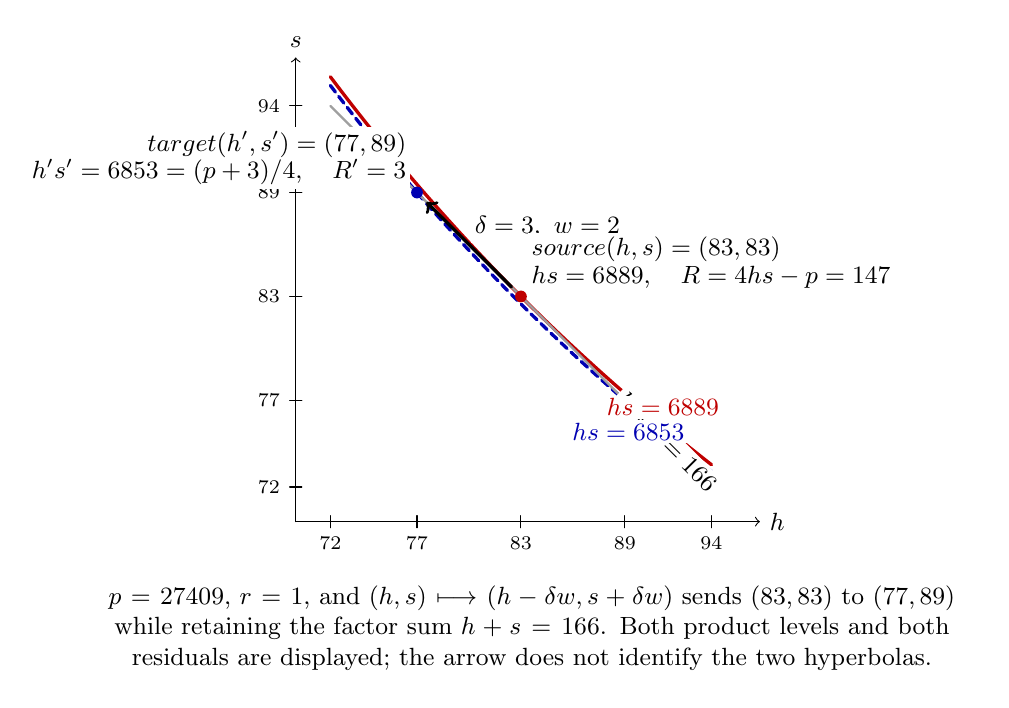
\begin{tikzpicture}[font=\small,line cap=round,line join=round]
  \begin{scope}[x=0.22cm,y=0.22cm,xshift=-15.4cm,yshift=-15.4cm]
    \draw[->] (70,70) -- (96.8,70) node[right] {$h$};
    \draw[->] (70,70) -- (70,96.8) node[above] {$s$};
    \foreach \x in {72,77,83,89,94}{
      \draw (\x,70.35) -- (\x,69.65)
        node[below] {\scriptsize $\x$};
      \draw (70.35,\x) -- (69.65,\x)
        node[left] {\scriptsize $\x$};
    }

    \draw[red!75!black,very thick]
      plot[domain=72:94,samples=100]
      (\x,{6889/\x});
    \draw[blue!70!black,very thick,densely dashed]
      plot[domain=72:94,samples=100]
      (\x,{6853/\x});
    \draw[gray!75,thick]
      plot[domain=72:94,samples=2]
      (\x,{166-\x});

    \fill[red!75!black] (83,83) circle[radius=0.34];
    \fill[blue!70!black] (77,89) circle[radius=0.34];
    \draw[->,black,very thick]
      (82.45,83.55) -- (77.55,88.45)
      node[midway,above right,fill=white,inner sep=1.5pt]
      {$\delta=3,\ w=2$};

    \node[above right,align=left,fill=white,inner sep=1.5pt]
      at (83.35,83.2)
      {$\text{source }(h,s)=(83,83)$\\[-1pt]
       $hs=6889,\quad R=4hs-p=147$};
    \node[above left,align=right,fill=white,inner sep=1.5pt]
      at (76.65,89.15)
      {$\text{target }(h',s')=(77,89)$\\[-1pt]
       $h's'=6853=(p+3)/4,\quad R'=3$};
    \node[rotate=-45,fill=white,inner sep=1pt]
      at (91.4,74.6) {$h+s=166$};
    \node[red!75!black,fill=white,inner sep=1pt]
      at (91.2,76.6) {$hs=6889$};
    \node[blue!70!black,fill=white,inner sep=1pt]
      at (89.2,75.2) {$hs=6853$};
  \end{scope}

  \node[align=center,text width=0.92\linewidth]
    at (3.0,-1.35)
    {$p=27409$, $r=1$, and
     $(h,s)\longmapsto(h-\delta w,s+\delta w)$ sends
     $(83,83)$ to $(77,89)$ while retaining the factor sum $h+s=166$.
     Both product levels and both residuals are displayed; the arrow does not
     identify the two hyperbolas.};
\end{tikzpicture}
\caption{The exact factor-sum arrow
$(h,s)\mapsto(h-\delta w,s+\delta w)$ on the first Pell-family example.
The source lies on $hs=6889$ and the target lies on $hs=6853$; their common
line is $h+s=166$.}
\label{fig:factor-sum-geometry}
\end{figure}


The general factor-sum map also works off the square carrier. At $p=12577$,
$a=3196$, $R=207$, $(h,r,s)=(47,1,68)$, one has $\delta=23,t=3,w=-1$.
The new factors are $70,45$, giving a full original state at residual 23.
The signed value of $w$ is essential; no positivity of the parameter $w$
is imposed in Theorem~\ref{thm:sumshift}.

\section{A second, distinct fibre: retain the numerical tail sum}\label{sec:tailsum}
The preceding map retains the raw factor sum $h+s$.  The next construction
retains instead the numerical tail sum $Y+Z$.  These are different functions
on the original state space, so we keep separate symbols, domains and inverse
conditions.

\begin{theorem}[Complete fixed-tail-sum fibre]\label{thm:tailsum}
Let $p$ be an odd prime, let $N>p$, and put
\[
 \mathcal D=N(N-p).
\]
Ordered positive integer triples satisfying
\[
 \frac4p=\frac1A+\frac1Y+\frac1Z,\qquad
 \frac p4<A<\frac p2,\qquad Y+Z=N
\]
are in bijection with pairs $(\rho,\Delta)\in\mathbb Z_{>0}\times\mathbb Z$
such that
\begin{equation}\label{eq:tailsum-gates}
 \begin{gathered}
  \rho\mid N,\qquad 0<\rho<p,\qquad \rho\equiv-p\pmod4,\\
  \Delta^2=\mathcal D-\frac{Np^2}{\rho},\qquad
  |\Delta|<N,\qquad \Delta\equiv N\pmod2.
 \end{gathered}
\end{equation}
The two mutually inverse coordinate maps are
\begin{equation}\label{eq:tailsum-inverse}
 \rho=4A-p,\quad \Delta=Z-Y;\qquad
 A=\frac{p+\rho}{4},\quad
 Y=\frac{N-\Delta}{2},\quad Z=\frac{N+\Delta}{2}.
\end{equation}
Consequently this fibre is decided by a finite divisor-and-square test.

Write uniquely $\rho=\delta v^2$, with $\delta$ positive and squarefree, and
put $X=v\Delta$.  The same fibre is the union of the exact lattice sections
\begin{equation}\label{eq:tailsum-pell}
\begin{aligned}
 X^2-\mathcal Dv^2&=-\frac{Np^2}{\delta},
 &\delta v^2&\mid N,\\
 X&\equiv Nv\pmod{2v},
 &0<\delta v^2&<p,
 &\delta v^2&\equiv-p\pmod4.
\end{aligned}
\end{equation}
Every condition in \eqref{eq:tailsum-pell} is part of the return map.  An
integer point on the displayed norm equation without the divisibility and
congruence conditions need not give integer tails.
\end{theorem}
\begin{proof}
Set $\rho=4A-p$.  The reciprocal identity and $Y+Z=N$ give
\[
 YZ=\frac{NpA}{\rho}=\frac{Np(p+\rho)}{4\rho}.
\]
Therefore
\[
 (Z-Y)^2=N^2-4YZ
 =N(N-p)-\frac{Np^2}{\rho},
\]
or, without a quotient,
\begin{equation}\label{eq:tailsum-discriminant}
 \rho\Delta^2=N\bigl((N-p)\rho-p^2\bigr).
\end{equation}
The first-half inequalities give $0<\rho<p$, while integrality of $A$ gives
$\rho\equiv-p\pmod4$.  Since $p$ is prime and $\rho<p$, one has
$\gcd(\rho,p)=1$; equation \eqref{eq:tailsum-discriminant} then forces
$\rho\mid N$.  Positivity and integrality of $Y,Z$ are exactly the final two
conditions in \eqref{eq:tailsum-gates}.  This proves necessity.  Substitution
of \eqref{eq:tailsum-inverse} proves the reciprocal identity and every range
condition, so it also proves sufficiency and both inverse compositions.

After $\rho=\delta v^2$, multiplication of the square equation by $v^2$
gives \eqref{eq:tailsum-pell}.  Conversely $v\mid X$ and
$X\equiv Nv\pmod{2v}$ recover an integer $\Delta=X/v$ with the required
parity.  The residual and range gates then recover exactly
\eqref{eq:tailsum-inverse}.  Thus the Pell lattice description loses no
coordinate and adds no candidate.
\end{proof}

There is an equivalent shifted-factor conic which makes the missing gate
visible.  Put
\[
 B=\rho Y-pA,\qquad C=\rho Z-pA,\qquad w=B-C.
\]
Then
\begin{equation}\label{eq:shifted-tail-conic}
 BC=(pA)^2,\qquad
 w^2=\mathcal D\rho^2-Np^2\rho.
\end{equation}
With
\[
 U=2\mathcal D\rho-p^2N,\qquad V=2w,
\]
equation \eqref{eq:shifted-tail-conic} becomes
\begin{equation}\label{eq:shifted-tail-pell}
 U^2-\mathcal D V^2=p^4N^2.
\end{equation}
However, exact integer tails require the additional gate
\begin{equation}\label{eq:shifted-tail-gate}
 \rho\mid w,\qquad
 Y=\frac12\left(N+\frac w\rho\right),\quad
 Z=\frac12\left(N-\frac w\rho\right).
\end{equation}
Thus the unrestricted Pell orbit in \eqref{eq:shifted-tail-pell} is a larger
space of shifted-factor points.  Its failure to land in
\eqref{eq:shifted-tail-gate} defines the exact return defect.

\begin{theorem}[Prime-square fixed-sum divisor obstruction]
\label{thm:prime-square-fixed-sum}
Let $p,q$ be odd primes satisfying
\[
 p\equiv1\pmod4,\qquad 2q^2<p<4q^2,
 \qquad R=4q^2-p.
\]
For $u\in\{q,q^3\}$ put
\[
 G_E(u)=4u+1,\qquad G_M(u)=p+4u.
\]
Choose $c\in\{E,M\}$ and suppose that the corresponding prime-square source
is a proper trace:
\[
 R\mid G_c(u)^2,\qquad R\nmid G_c(u).
\]
Let $(y,z)$ be its ordered rational tails from
\eqref{eq:E} or \eqref{eq:M}, and set $N=y+z\in\mathbb Z$.
There is no positive integral target
\[
 \frac4p=\frac1A+\frac1Y+\frac1Z,\qquad Y+Z=N,
\]
whose residual $S=4A-p$ is a proper divisor of the source residual:
\[
 S\mid R,\qquad 0<S<R.
\]
The target may change the word, the E/M channel and the tail order.
\end{theorem}
\begin{proof}
The source data can be kept without suppressing any of the four marked
states.  Define $H$ by the following table:
\begin{equation}\label{eq:prime-square-source-table}
\begin{array}{c|c|c|c}
(c,u)&H&(y,z)&N\\ \hline
(E,q)&p+q&
\left(q^2H/R,pqH/R\right)&qH^2/R\\[1mm]
(E,q^3)&pq+1&
\left(qH/R,pq^2H/R\right)&qH^2/R\\[1mm]
(M,q)&q+1&
\left(pq^2H/R,pqH/R\right)&pqH^2/R\\[1mm]
(M,q^3)&q+1&
\left(pqH/R,pq^2H/R\right)&pqH^2/R .
\end{array}
\end{equation}
The trace gates transfer to $H$ because
\[
\begin{aligned}
 H&=qG_E(q)-R &&(E,q),\\
 H&=G_E(q^3)-qR &&(E,q^3),\\
 G_M(q)&=4qH-R &&(M,q),\\
 G_M(q^3)&=qR+pH &&(M,q^3).
\end{aligned}
\]
Every displayed multiplier is a unit modulo $R$, since
$\gcd(R,pq)=1$.  Hence
\[
 R\mid H^2,\qquad R\nmid H.
\]

Put
\[
 g=\gcd(R,H),\qquad \eta=R/g,\qquad F=H/g.
\]
Then $\gcd(\eta,F)=1$.  The divisibility $R\mid H^2$ forces
$\eta\mid g$; write
\begin{equation}\label{eq:prime-square-canonical}
 g=k_0\eta,\qquad
 R=k_0\eta^2,\qquad H=k_0\eta F.
\end{equation}
Here $k_0$ is a local gcd factor and is not the least square modulus $K$
used in Sections~\ref{sec:defect}--\ref{sec:squares}.  Properness is exactly
$\eta>1$.  Since $R$ is odd, $\eta\ge3$, and
\[
 \gcd(\eta,pqF)=1.
\]
In every row of \eqref{eq:prime-square-source-table}, neither $p$ nor $q$
divides $H$; also $k_0\mid R$.  Hence
\begin{equation}\label{eq:pq-coprime-source}
 \gcd(pq,k_0F)=1.
\end{equation}
The four source sums in \eqref{eq:prime-square-source-table} therefore become
\begin{equation}\label{eq:prime-square-source-sum}
 N=
 \begin{cases}
 qk_0F^2,&c=E,\\
 pqk_0F^2,&c=M,
 \end{cases}
 \qquad\text{and}\qquad
 \gcd(R,N)=k_0.
\end{equation}

Assume that a target with $S\mid R$ and $0<S<R$ exists.  Its first
denominator satisfies the exact chain
\[
 A=\frac{p+S}{4}<\frac{p+R}{4}=q^2<\frac p2.
\]
In particular $p\nmid A$.  Also
$S\equiv-p\equiv3\pmod4$, so $S$ is odd and $S\ge3$.  From the target
identity and $Y+Z=N$,
\[
 YZ=\frac{NpA}{S}.
\]
One has $\gcd(S,pA)=1$: a common divisor of $S$ and $A$ divides
$4A-S=p$, while $S<p$.  Thus $S\mid N$, and
\begin{equation}\label{eq:S-divides-k0}
 S\mid\gcd(R,N)=k_0.
\end{equation}

The complete inverse in Lemma~\ref{lem:trace}, applied at residual $S$,
shows that after the required E tail orientation the target has exactly one
of the following two forms, with $\gcd(r,s)=1$:
\begin{align}
 E:\quad&
 A=hrs,\quad S\kappa=pr+s,\quad
 (Y,Z)=(hs\kappa,phr\kappa),\quad
 N=hS\kappa^2,\label{eq:target-E-fixed-sum}\\
 M:\quad&
 A=hrs,\quad S\lambda=r+s,\quad
 (Y,Z)=(phs\lambda,phr\lambda),\quad
 N=phS\lambda^2.\label{eq:target-M-fixed-sum}
\end{align}
All displayed parameters are positive integers.  Because $p\nmid hS$, the
$p$-adic valuation of an E target sum is even and that of an M target sum is
odd.  Equation \eqref{eq:prime-square-source-sum} has valuation zero in the
source E channel and one in the source M channel.  Therefore the target
channel equals the source channel.

Let $\theta=\kappa$ in E and $\theta=\lambda$ in M.  Comparing target and
source sums and using \eqref{eq:S-divides-k0} gives
\begin{equation}\label{eq:prime-square-sum-comparison}
 q\frac{k_0}{S}F^2=h\theta^2.
\end{equation}
The prime $q$ divides neither $(k_0/S)$ nor $F$, while $h\mid A<q^2$.
Taking $q$-adic valuations in
\eqref{eq:prime-square-sum-comparison} yields
\[
 h=qh_0,\qquad q\nmid h_0\theta.
\]
Consequently $q\mid A$.  There is a unique integer $j$ with
\begin{equation}\label{eq:prime-square-j}
 A=q(q-j),\qquad 0<j<q,\qquad R-S=4qj,
\end{equation}
and cancellation of $q$ in
\eqref{eq:prime-square-sum-comparison} gives
\begin{equation}\label{eq:prime-square-reduced-comparison}
 \frac{k_0}{S}F^2=h_0\theta^2.
\end{equation}

There are three cases after the two M orientations are kept together.

\emph{Case $E,u=q$.}
Here $H=p+q=k_0\eta F$.  From
\eqref{eq:prime-square-reduced-comparison},
\[
 \kappa\le F\sqrt{\frac{k_0}{S}},
 \qquad
 S\kappa\le F\sqrt{Sk_0}\le Fk_0
 =\frac{p+q}{\eta}<p.
\]
But the exact E gate in \eqref{eq:target-E-fixed-sum} gives
$S\kappa=pr+s>p$, a contradiction.

\emph{Cases $M,u=q$ and $M,u=q^3$.}
In both cases $H=q+1=k_0\eta F$, hence $q=k_0\eta F-1$.
Using \eqref{eq:prime-square-j},
\[
 k_0\eta^2-S=4j(k_0\eta F-1),
\]
or
\begin{equation}\label{eq:M-multiple-obstruction}
 k_0\eta(\eta-4jF)=S-4j.
\end{equation}
The right side is nonzero because $S$ is odd.  Moreover
$0<S\le k_0<k_0\eta$.  Since $k_0$ and $\eta$ are odd while
$q+1=k_0\eta F$ is even, $F$ is even and $k_0F\ge2$, so
$q\ge2\eta-1>\eta$.  It follows that
\[
 0<4j=\frac{R-S}{q}<\frac Rq
 =\frac{k_0\eta^2}{q}<k_0\eta.
\]
Thus $0<|S-4j|<k_0\eta$, contradicting
\eqref{eq:M-multiple-obstruction}, which makes $S-4j$ a nonzero multiple of
$k_0\eta$.

\emph{Case $E,u=q^3$.}
Here $H=pq+1=k_0\eta F$.  Reduce $\kappa/F$ to lowest terms by writing
\[
 F=nw,\qquad \kappa=mw,\qquad \gcd(m,n)=1.
\]
Equation \eqref{eq:prime-square-reduced-comparison} gives a positive integer
$\tau$ such that
\[
 \frac{k_0}{S}=\tau m^2,\qquad h_0=\tau n^2.
\]
Set $\Gamma=\tau m\eta n$.  Then the source identity and the exact target
gate give
\[
 pq+1=k_0\eta F
 =\Gamma S\kappa
 =\Gamma(pr+s),
\]
so
\begin{equation}\label{eq:Gamma-congruence}
 \Gamma s\equiv1\pmod p.
\end{equation}
From \eqref{eq:prime-square-j},
$q-j=h_0rs=\tau n^2rs$, and hence
\[
 0<\tau ns=\frac{q-j}{nr}<q.
\]
Also
\[
 R=S\tau(m\eta)^2<2q^2.
\]
The already retained congruence $S\equiv3\pmod4$ gives $S\ge3$; therefore
\[
 (m\eta)^2<\frac{2q^2}{3}<q^2.
\]
It follows that
\[
 0<\Gamma s=(m\eta)(\tau ns)<q^2<p.
\]
Together with \eqref{eq:Gamma-congruence}, this forces $\Gamma s=1$, whereas
$\Gamma s\ge\eta\ge3$.  This final contradiction exhausts all four marked
prime-square sources.
\end{proof}

The divisor hypothesis in Theorem~\ref{thm:prime-square-fixed-sum} is part
of its scope.  It does not exclude a smaller residual $S<R$ with
$S\nmid R$, and it does not apply after changing the numerical tail sum
$N$.  It is also separate from the composite-carrier obstruction below.

At $p=67369$, the proper M trace
\[
 (a,R,u,h,r,s)=(16849,27,1421,29,7,83)
\]
has ordered rational tails
\[
 (y,z)=\left(\frac{1621571830}{3},\frac{136759070}{3}\right),\qquad
 N=586110300.
\]
Its shifted factors are
\[
 (B,C,w)=(13459046189,95731349,13363314840),\qquad
 w\equiv18\pmod{27}.
\]
It therefore supplies an exact integer point of
\eqref{eq:shifted-tail-pell}, but not an integer-tail return.  The complete
list allowed by \eqref{eq:tailsum-gates} before the square test is
\[
 \rho\in\{3,15,75,87,435,2175\}.
\]
For $\rho=3$ the discriminant is negative.  For the remaining five residuals
it is respectively $2$ modulo $3$, $5$ modulo $7$, $2$ modulo $3$, $3$
modulo $7$, and $2$ modulo $3$.  Each is a quadratic nonresidue, so this
source has no integral target anywhere in its fixed numerical tail-sum fibre.

The complete first-half census at this prime has 69 proper original trace tags
with 51 distinct numerical tail sums, and 47 integral tags with 37 distinct
tail sums.  The two sets of sums are disjoint.  Applying
Theorem~\ref{thm:tailsum} to all 51 proper sums produces 507 eligible residual
divisors; 478 have nonnegative discriminant and none has a square
discriminant.  The separately written checker recomputes the divisor lists,
tail sums and square tests without importing the main implementation.  This is
a fixed-prime structural obstruction to retaining $Y+Z$, not a counterexample
to Erd\H{o}s--Straus and not a failure of the factor-sum map of
Theorem~\ref{thm:sumshift}.

\section{A least obstruction to universal nonincreasing trace repair}\label{sec:prefix}
\begin{theorem}[Finite least example]\label{thm:least}
Let $A_{\mathrm{tr}}(p)$ and $A_{\mathrm{full}}(p)$ be the least first-half
distinguished denominators supporting, respectively, an original trace and
an original full state; use $+\infty$ for an empty set. Among primes
$p\equiv1\pmod{24}$, the least with
$A_{\mathrm{tr}}(p)<A_{\mathrm{full}}(p)$ and $A_{\mathrm{tr}}(p)<+\infty$ is
\[
 p=67369.
\]
Its first trace shell has $a=16849=7\cdot29\cdot83$, $R=27$; its first full
shell has $a=16850$, $R=31$. Thus no universal map from \emph{every} original
rational trace to an integral witness at the same prime can require $a'\le a$.
\end{theorem}
\begin{proof}[Deterministic finite proof]
The certificate enumerates all 817 primes congruent to one modulo 24 through
67369 by a sieve and independently verifies that list. For each it enumerates
consecutive original shells from $R=3$ through the first full shell, factoring
$a$ and listing the complete divisors of $a^2$. For every smaller prime, the
first trace shell already has a full gate; thus every trace at that prime has
some full witness with distinguished denominator no larger than its own.
Exactly at 67369 the first trace precedes the first full gate.

For that prime, every word and both gate residues are serialized for
$R=3,7,11,15,19,23,27,31$. The first six have no traces. At $R=27$, the four
E trace words are $29,83,488621,1398467$, and the four M trace words are
$1421,4067,69803,199781$. All are proper. At $R=31$, $a=16850=2\cdot5^2\cdot337$
has the two E words $674,84250$. The full enumeration and the independent
rational-tail test agree on these lists.

The short first-half completeness argument below ensures that this excludes
all integral witnesses with smaller distinguished denominator, not merely a
preferred subfamily of states. Integer sieve, factorization and finite loops
make the computation an executable exhaustive proof with the stated bound.
No leastness claim beyond that checked prime class is made.
\end{proof}

For completeness, every positive integer witness at an odd prime
$p\equiv1\pmod4$ has a first-half distinguished denominator. At least one
and at most two denominators are divisible by $p$. With two, the remaining
unit denominator has reciprocal strictly greater than $2/p$, hence lies below
$p/2$; it is above $p/4$ by positivity. With one, write that denominator $pk$
and the other two $a=gr\le b=gs$, $\gcd(r,s)=1$. They are units at $p$.
The equation gives $p\mid4k-1$, so $4k-1=pt$ with $t\equiv3\pmod4$.
It reduces to $tgrs=k(r+s)$. Hence $k=jrs$, $r+s=t\lambda$, and
$g=j\lambda$, since $\gcd(t,k)=1$.
If $a\ge p/2$, then $2jr(r-s)\ge-1$; its even nonpositive left side forces
$r=s=1$, contradicting $t\mid2$. Thus $p/4<a<p/2$.
The factor-pair argument of Lemma~\ref{lem:trace}, now with integral tails,
then recovers a full original E/M word.

The least-example theorem does not contradict the successful strict descents
above. It says that their domains cannot be extended to every trace merely
by improving their choice of descending word. At this prime a general repair
must sometimes move to a larger distinguished denominator, or start from a
different trace already above the first occupied shell.

\section{Counterfactual constraints and the next exact obligation}
For an arbitrary prescribed prime $p\equiv1\pmod{24}$, the construction of
Sections~\ref{sec:defect}--\ref{sec:tiles} is finite on every original shell.
If all full gates failed, then every squarefree shell would have no trace;
every coarse trace part at a squareful shell would have zero coefficient
\eqref{eq:tilepoly}; in particular its unit-direction width would be at most
$D-2$. Every oriented M trace would fail the exact integer-root test
\eqref{eq:quad}, because a passing root constructs a genuine full state at
the same prime. On a prime-power M source, $e<bd_b$ would be necessary.
These are proved simultaneous necessary conditions in the original bounded
arrays. They do not contradict one another by assumption.

The next missing implication is an arithmetic incompatibility of those
complete zero coefficients across different shells, or another explicit
source-changing mechanism that forces a full coefficient. The prefix example
rules out universal nonincrease of $a$ as its sole termination invariant.
Receiver nonvanishing is not invoked as initial-source positivity. Neither a
nonempty subgroup nor a limit of averages is substituted for an original word.

\section{Computation, reproducibility and scope}
The main standard-library verifier scans every original word at all 143
primes $p\equiv1\pmod{24}$ through 10000: 171732 shells and 5616298 words.
Its exact trace counts are 5788 E and 5678 oriented M; full counts are 3637 E
and 3910 M. It reconstructs 4139 additive parts over 2522 squareful trace
shells and compares all coefficients with direct original gates.
The prime-square scan through $p\le2000000$ contains 167 occupied trace
shells and 285 marked states: E has 52 full and 83 proper; M has 56 full and
94 proper. These are source-state counts, not new primes solved globally.
The prefix proof covers 817 primes and 1422 tested shells. The main prime-square
lane generates candidate residuals from the three explicit squared linear
forms; the separate lane instead scans the whole prime interval for each
prime square and tests rational tail sums.

The separate implementation imports neither the main verifier nor its arithmetic
module. It checks the full source census, every additive part, all prime-square
sources, every prefix gate and every displayed arrow and its incoming fibre.
It is a separately written check, not independent human peer review.
Run \texttt{python run\_all.py --directory reproduced} for normal, optimized,
and separate lanes. Every failure raises an exception even under optimized
Python; integer coefficients are never stored as floating-point numbers.
The manifest and execution receipt record actual file hashes and observed runs.
The universal proofs use the displayed ring, valuation, finite sumset and
quadratic identities. Finite tests corroborate those proofs; the finite
leastness statement is explicitly computational.

No Lean build, historical-priority determination or universal ES proof is
claimed. The supplied Lean plan lists exact theorem dependencies. The original
source, ordered maps, finite fibres and all exceptional tests remain available
in \texttt{arithmetic.py}, \texttt{MORPHISMS.md}, and the JSON tables.
